%---------------------------------- Hertz ODR -----------------------------
\section{Hertz method with ODR} \label{hertz_odr}
This is a modification of the Hertz method explained in section \ref{hertz} and uses orthogonal distance regression. 
The loading curve is fitted with a more general power function but the relationship between the proportionality coefficient and the radius and modulus is assumed to stay the same.
If the resulting power differs from the theoretical value 1.5, this is an indicator that the Hertzian model is not adequate. The results for radius or modulus in this case do not make any physical sense.\\
This method is shown unless the software was compiled without Fortran support.  \\

\begin{figure}[ht]
  \centering
  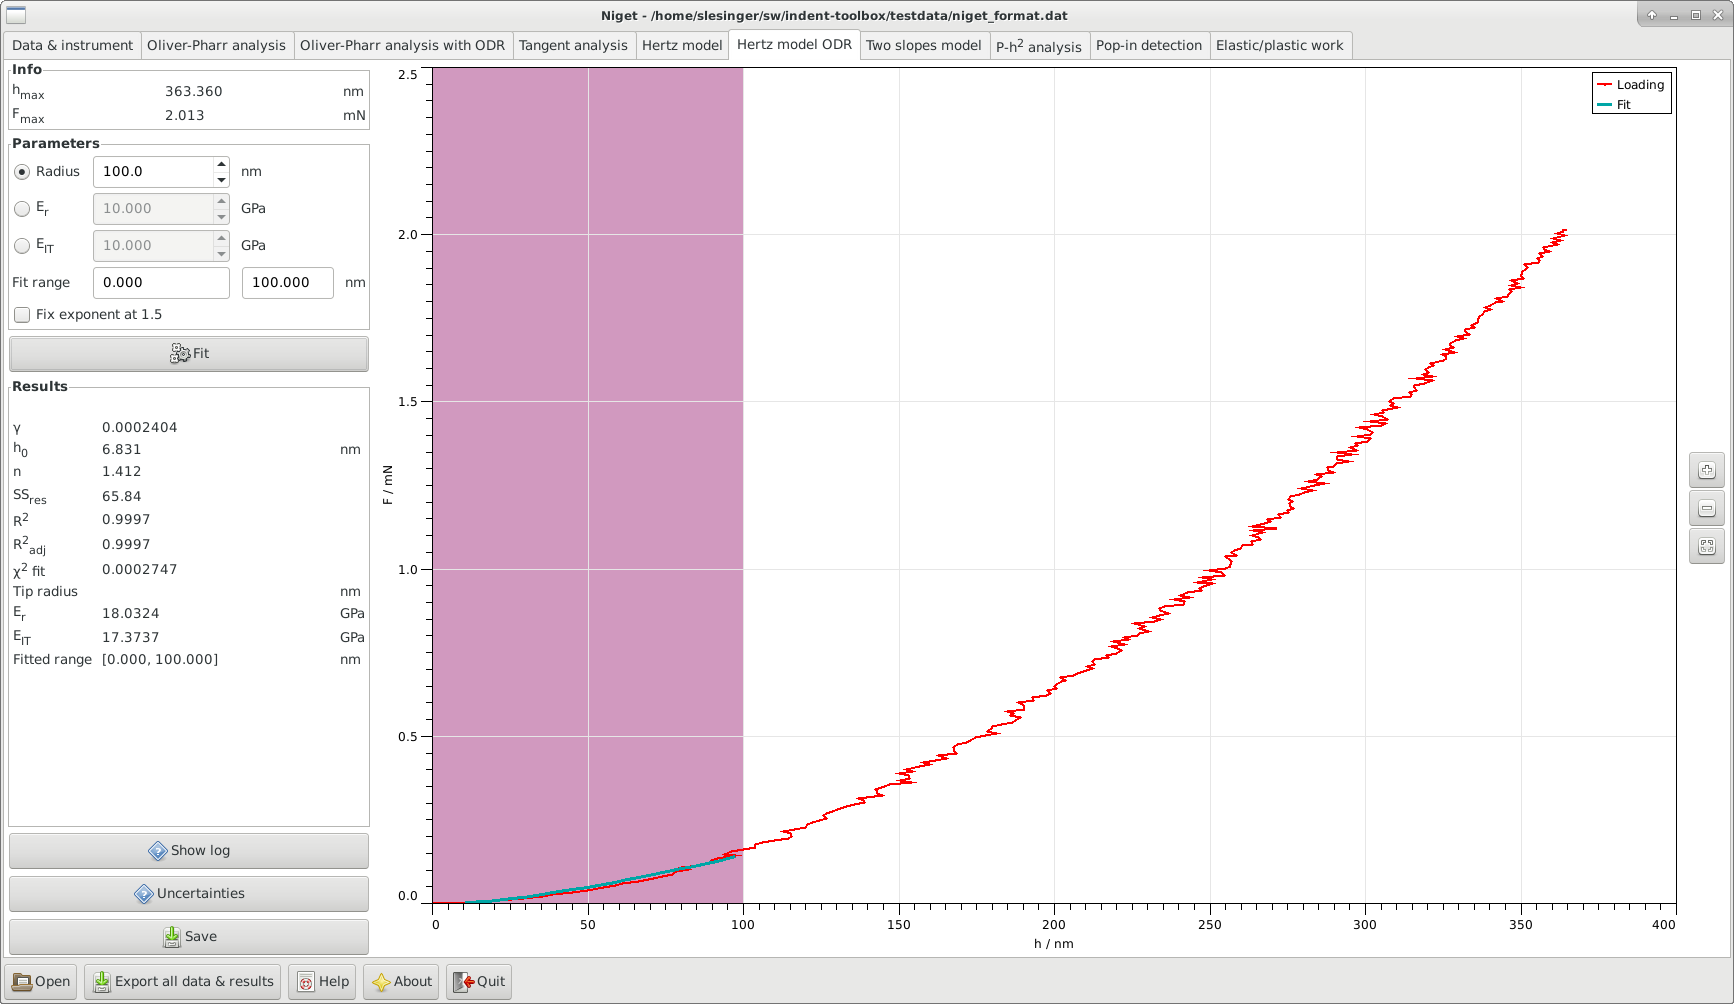
\includegraphics[width=\textwidth]{images/screen-hertz-odr}
  \caption{Hertzian model with ODR analysis}
\end{figure}

\subsection{Window}
The window consists of several blocks:
\begin{itemize}
 \item \emph{Info} displays the maximum depth and force during the indentation
 \item \emph{Parameters} shows the selected range in nm. 
        \begin{itemize}
           \item[-] The input variable can be chosen to be either the tip radius, the reduced modulus or the indentation modulus and its value should be set accordingly.
           \item[-] The fitting range can be selected either using the mouse or typing in the range entries. The range must be chosen so that the behavior remains elastic and the fit adequate.
           \item[-] Check box, whether or not the exponent should be fitted or fixed at the value 1.5, see \ref{hertz_odr_calc}.
        \end{itemize}
 \item \emph{Fit} button, see section \ref{hertz_odr_calc} for details of the calculation.
 \item \emph{Results} displays the results and the ranges used for the fitting procedure. 
       The variables are described in detail in section \ref{hertz_odr_calc}.
 \item \emph{Show log} Show the report about the fitting procedure in a separate window.  The reports are saved to files \emph{fit.log.hz.err} and \emph{fit.log.hz.rpt}.
 \item \emph{Uncertainties} show the uncertainty analysis window, see section \ref{hertz_odr_unc}.
 \item \emph{Save} save parameters and results to given file. 
 \item \emph{Graph} display the unloading curve and the fitted curves.  Stepwise zooming/unzooming can be performed by selecting a range with the mouse and pressing the \emph{Zoom}/ \emph{Unzoom} buttons. The graph is restored to its original size by the \emph{Restore} button.
\end{itemize}

\subsection{Procedure} \label{hertz_odr_calc}
\begin{enumerate} 
 \item 
The Hertzian model \eqref{eq:hertzfit} is fitted with a more general function 
\begin{equation} \label{eq:hertzodrfit}
F = \gamma  (h - h_0)^{n},  
\end{equation}
using orthogonal least squares implemented in ODRPACK. 
The power $n$ can be fixed at the theoretical value 1.5.
\item  
Further steps are the same as steps 2--4 in section \ref{hertz_calc} with $\gamma$ used instead of $a$. 
\end{enumerate}
